\documentclass[9pt]{beamer}

\usepackage{siunitx}
\usepackage{calc}
\usepackage{textpos}
\usepackage{physics}
\usepackage{amsmath}
\usepackage{tikz}
\usepackage{xparse}% So that we can have two optional parameters
\usepackage{mathtools}
\usepackage{eso-pic}
\usepackage{mdframed}
\usepackage{newunicodechar}
\usepackage[justification=centering]{caption}
\usepackage{subfig}

% Select font
%\usefonttheme{sf}
\setbeamerfont{title}{size=\huge,series=\bfseries,parent=structure,family=\fontfamily{\sfdefault}\selectfont}
\setbeamerfont{subtitle}{size=\Large,series=\bfseries,parent=structure, family=\fontfamily{\sfdefault}\selectfont}
\setbeamerfont{frametitle}{size=\LARGE,   family=\fontfamily{\sfdefault}\selectfont,series=\bfseries}
\setbeamerfont{framesubtitle}{size=\large,family=\fontfamily{\sfdefault}\selectfont,series=\normalfont}
\setbeamerfont{author}{size=\large,series=\bfseries,parent=structure,family=\fontfamily{\sfdefault}\selectfont}
\setbeamerfont{date}{size=\normalsize,series=\bfseries,parent=structure,family=\fontfamily{\sfdefault}\selectfont}
    
    
\beamertemplatenavigationsymbolsempty

\NewDocumentCommand\DownArrow{O{2.0ex} O{black}}{%
	\mathrel{\tikz[baseline] \draw [<-, line width=0.5pt, #2] (0,0) -- ++(0,#1);}
}
\NewDocumentCommand\UpArrow{O{2.0ex} O{black}}{%
	\mathrel{\tikz[baseline] \draw [->, line width=0.5pt, #2] (0,0) -- ++(0,#1);}
}

\newcommand\Warning{%
	\makebox[1.4em][c]{%
		\makebox[0pt][c]{\raisebox{.1em}{\small!}}%
		\makebox[0pt][c]{\color{red}\Large$\bigtriangleup$}
	}
}%

\newunicodechar{⚠}{\Warning}


\usetheme{Madrid}

\colorlet{beamer@blendedblue}{red!65!black}


\title[\fontfamily{\sfdefault}\selectfont Spatial monitoring of anti-vaccine opinions]{
	
\includegraphics[height=2cm]{images/logo/unipd_logo_white.png}\\
	~\\
	\textbf{
		Spatial monitoring of anti-vaccine opinions through Twitter: a method proposal
	}
}
\subtitle{\fontfamily{\sfdefault}\selectfont Life Data Epidemiology}
\author[\fontfamily{\sfdefault}\selectfont Favaretto, Lambertini, Pagano]{Rachele Favaretto, Alessandro Lambertini, Alice Pagano}
\date{\fontfamily{\sfdefault}\selectfont February 15, 2021}



% Modify Frametitle
\addtobeamertemplate{frametitle}{}{%
	\begin{textblock*}{100mm}(.85\textwidth,-1.1cm) %before -0.9cm
		
\includegraphics[height=0.85cm]{images/logo/unipd_logo_white.png}
	\end{textblock*}
}



\begin{document}

	\maketitle

%	\begin{frame}{Outline}
%		\framesubtitle{~}
%
%		\tableofcontents
%		
%	\end{frame}

	%% 1: Introduction
	%% 2: Experimental Setup
	%% 3: Commissioning measurements
	%% 4: Measurements of the tritium beta-spectrum
	%% 5: Data Analysis
	%% 6: Results
	%% 7: Conclusion and outlook


	\section{Introduction}
	
	\begin{frame}[c]{Introduction}
	\framesubtitle{The idea behind the project}

	\boxed{\textbf{Observation}}
	\medskip
	
    \alert{Anti-vaccine opinions} represent a \alert{challenge} for \alert{health care systems} in many countries all around the world
    
    \medskip
    
    $\implies$ to solve this issue \alert{information campaigns} are needed. 
    
    \medskip 
    
    These measures are long-term effective, but immediately \alert{expensive}
    
    \medskip
    
    $\implies$ useful to find a way to \alert{optimize} the \alert{allocation of resources}.
	
	\medskip
	\medskip
	\medskip
	
	\pause
	
	\boxed{\textbf{Solution}}
	\medskip
	
	\alert{Vaccination} has become a \alert{central topic} in public debate on \alert{social networks} 
	
	\medskip
	
	$\implies$ use social networks to \alert{spatial monitor opinions} in a given territory.
	
	\end{frame}
	
%	\begin{frame}{Introduction}
%	\framesubtitle{Outline}
%    \begin{itemize}
%        \item 
% 
%	\end{frame}
	
	
	\section{Methods}
	
	\begin{frame}{Methods}
	\framesubtitle{Collecting and pre-processing the data}
    \begin{figure}[t]
	    \begin{minipage}[l]{1\columnwidth}
	    \centering
	    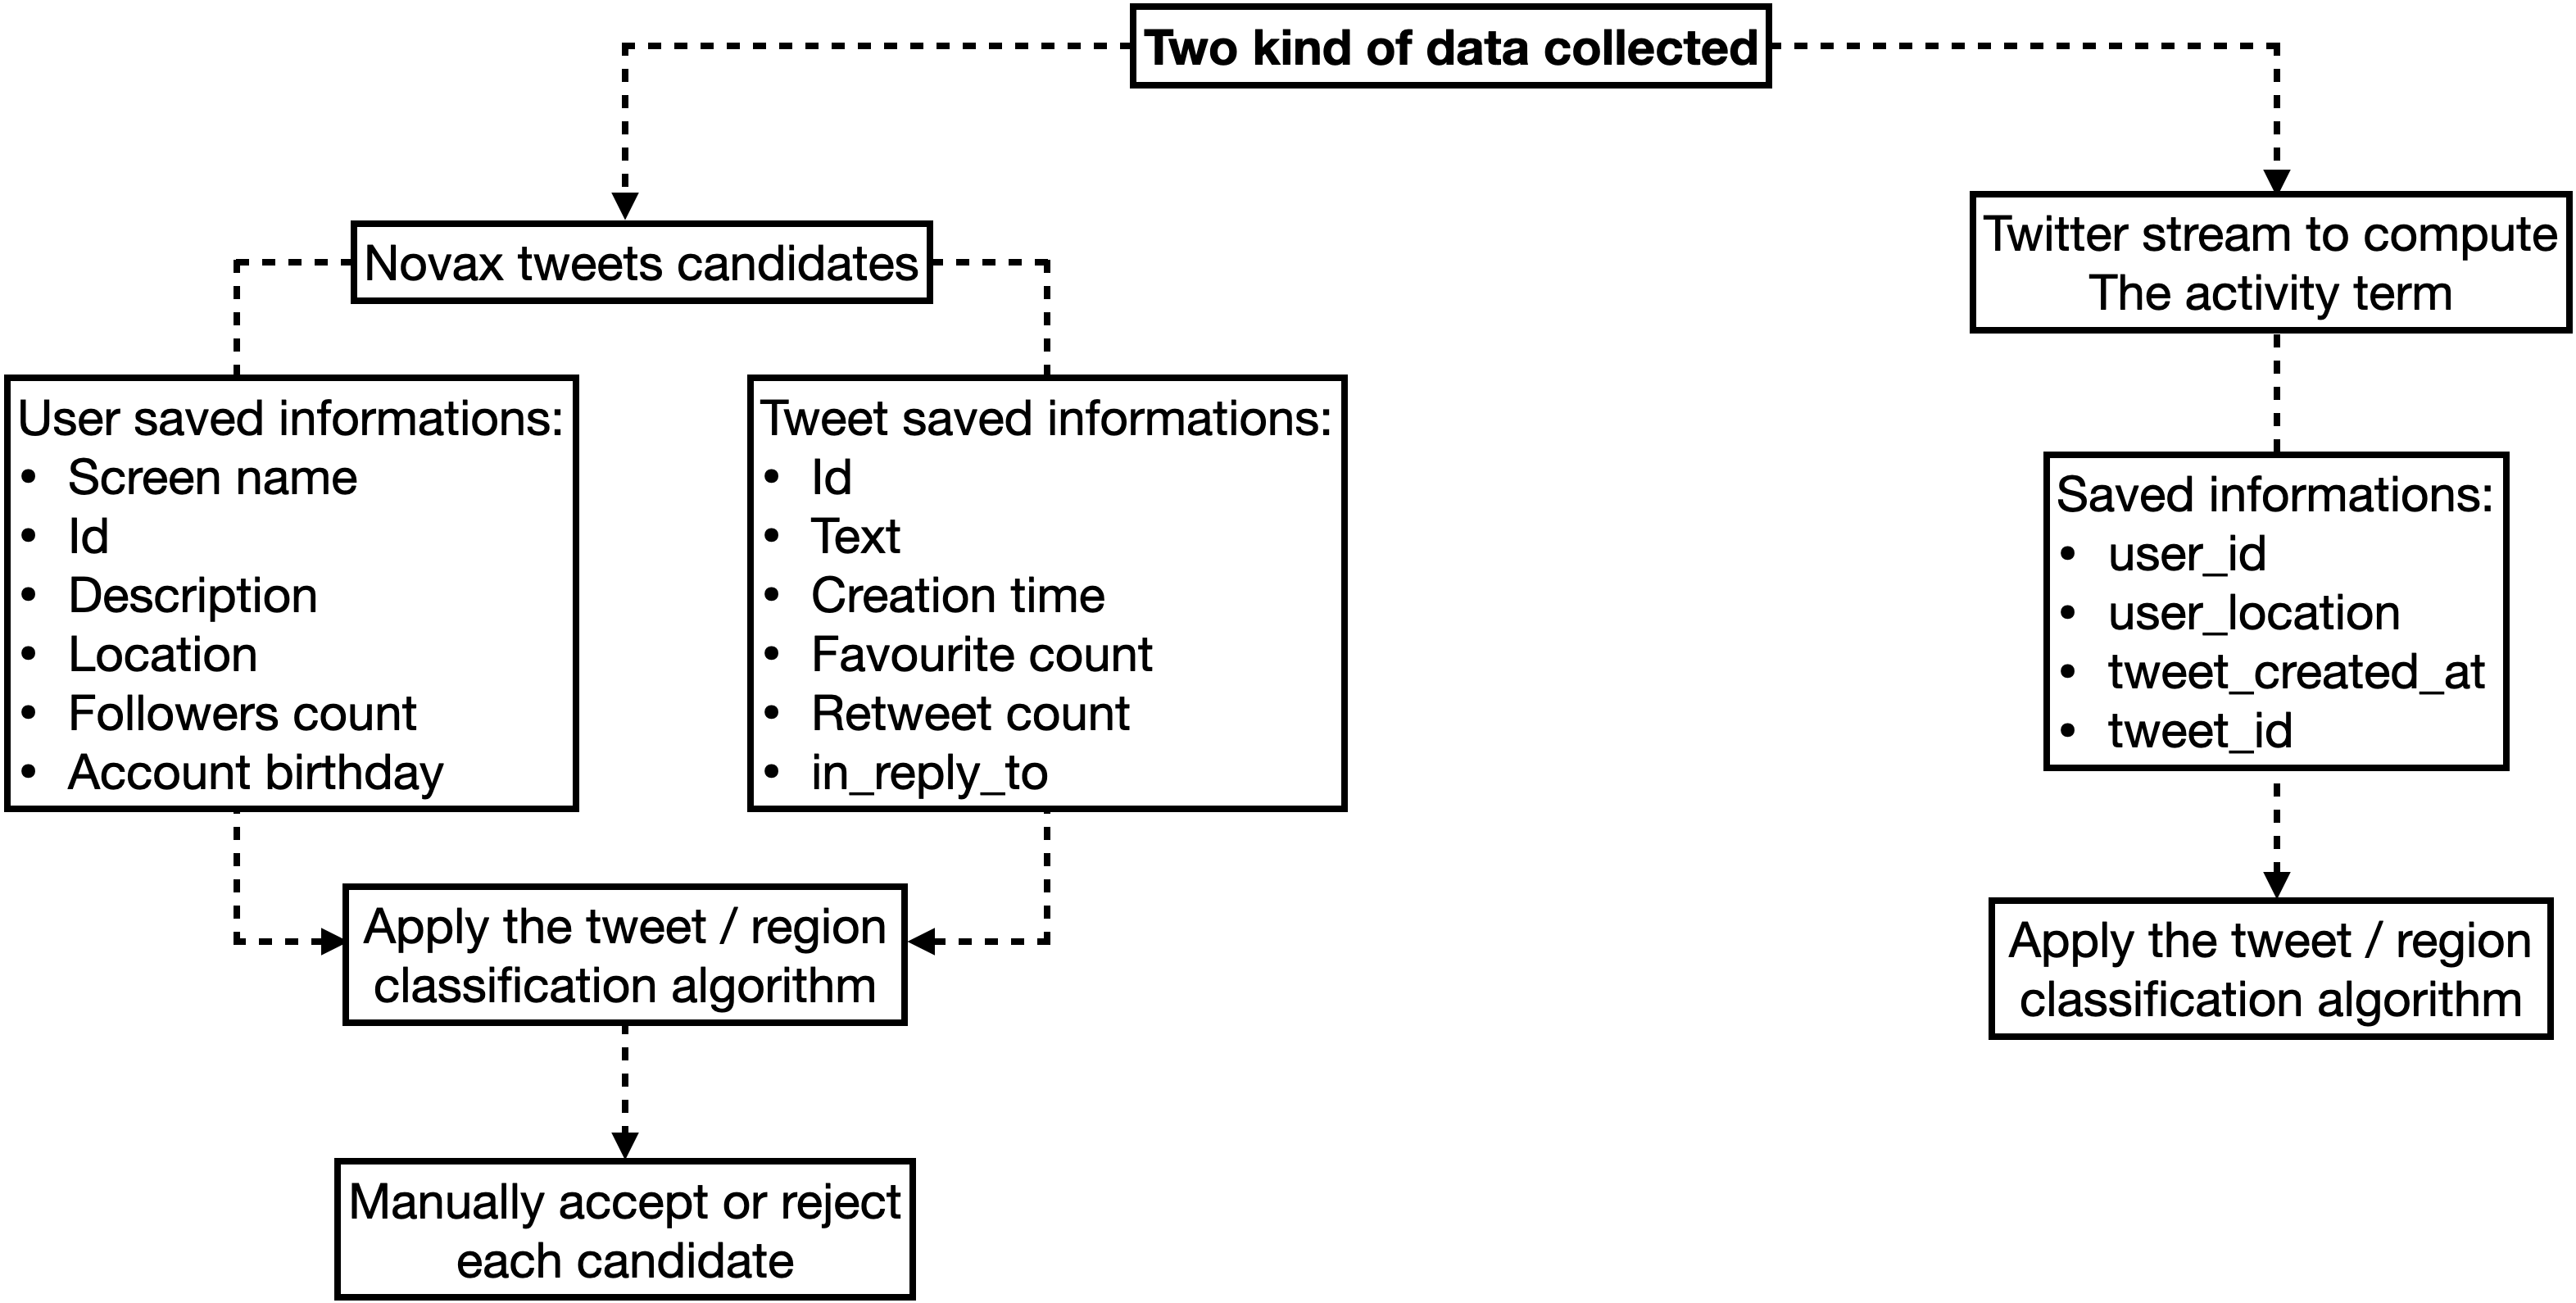
\includegraphics[width=1\textwidth]{images/schema2.png}
        \label{fig:}
        \end{minipage}
    \end{figure}
	\end{frame}
	
	\begin{frame}{Methods}
	\framesubtitle{Datasets dimensions}
	
	\centering
	\boxed{\textbf{Novax dataset}}
	\medskip
	
    \begin{table}[b]
    \begin{minipage}[l]{0.7\textwidth}
    \centering
        \begin{tabular*}{\linewidth}{@{\extracolsep{\fill}}
        l cccc 
        }
       %\toprule
            & \textbf{2017} & \textbf{2018} &  \textbf{2019} & \textbf{2020} \\
        \colrule
            $\pmb{d_t}$    & 438 & 405 & 382 & 277 \\
       % \colrule
            $\pmb{d_{nv}}$ & 83.3 \% & 88.6 \% & 98.2 \% & 82.3 \% \\
       % \colrule
            $\pmb{d_{u}}$  & 22.5 \% & 32.3 \% & 39.2 \% & 59.2 \% \\
       %\botrule
        \end{tabular*}
    \label{tab:dataset_dimension}
    \end{minipage}
    \caption{Dataset dimension for the different years under study. $d_t$ is the total dimension of the tweet dataset after location classification. $d_{nv}$ is the percentage of $d_t$ of tweets that express actually a novax opinion. $d_u$ is the percentage of unique users of $d_{nv}$. }
    \end{table}
    
    \medskip
    \medskip
    
    \pause
    
    \centering
	\boxed{\textbf{Twitter Activity dataset}}
	\medskip
    
    Around 48k geolocalized tweets of 7k unique users.
    
	\end{frame}
	
	\begin{frame}{Methods}
	\framesubtitle{Processing the data}
		    \begin{figure}[t]
	    \begin{minipage}[l]{1\columnwidth}
	    \centering
	    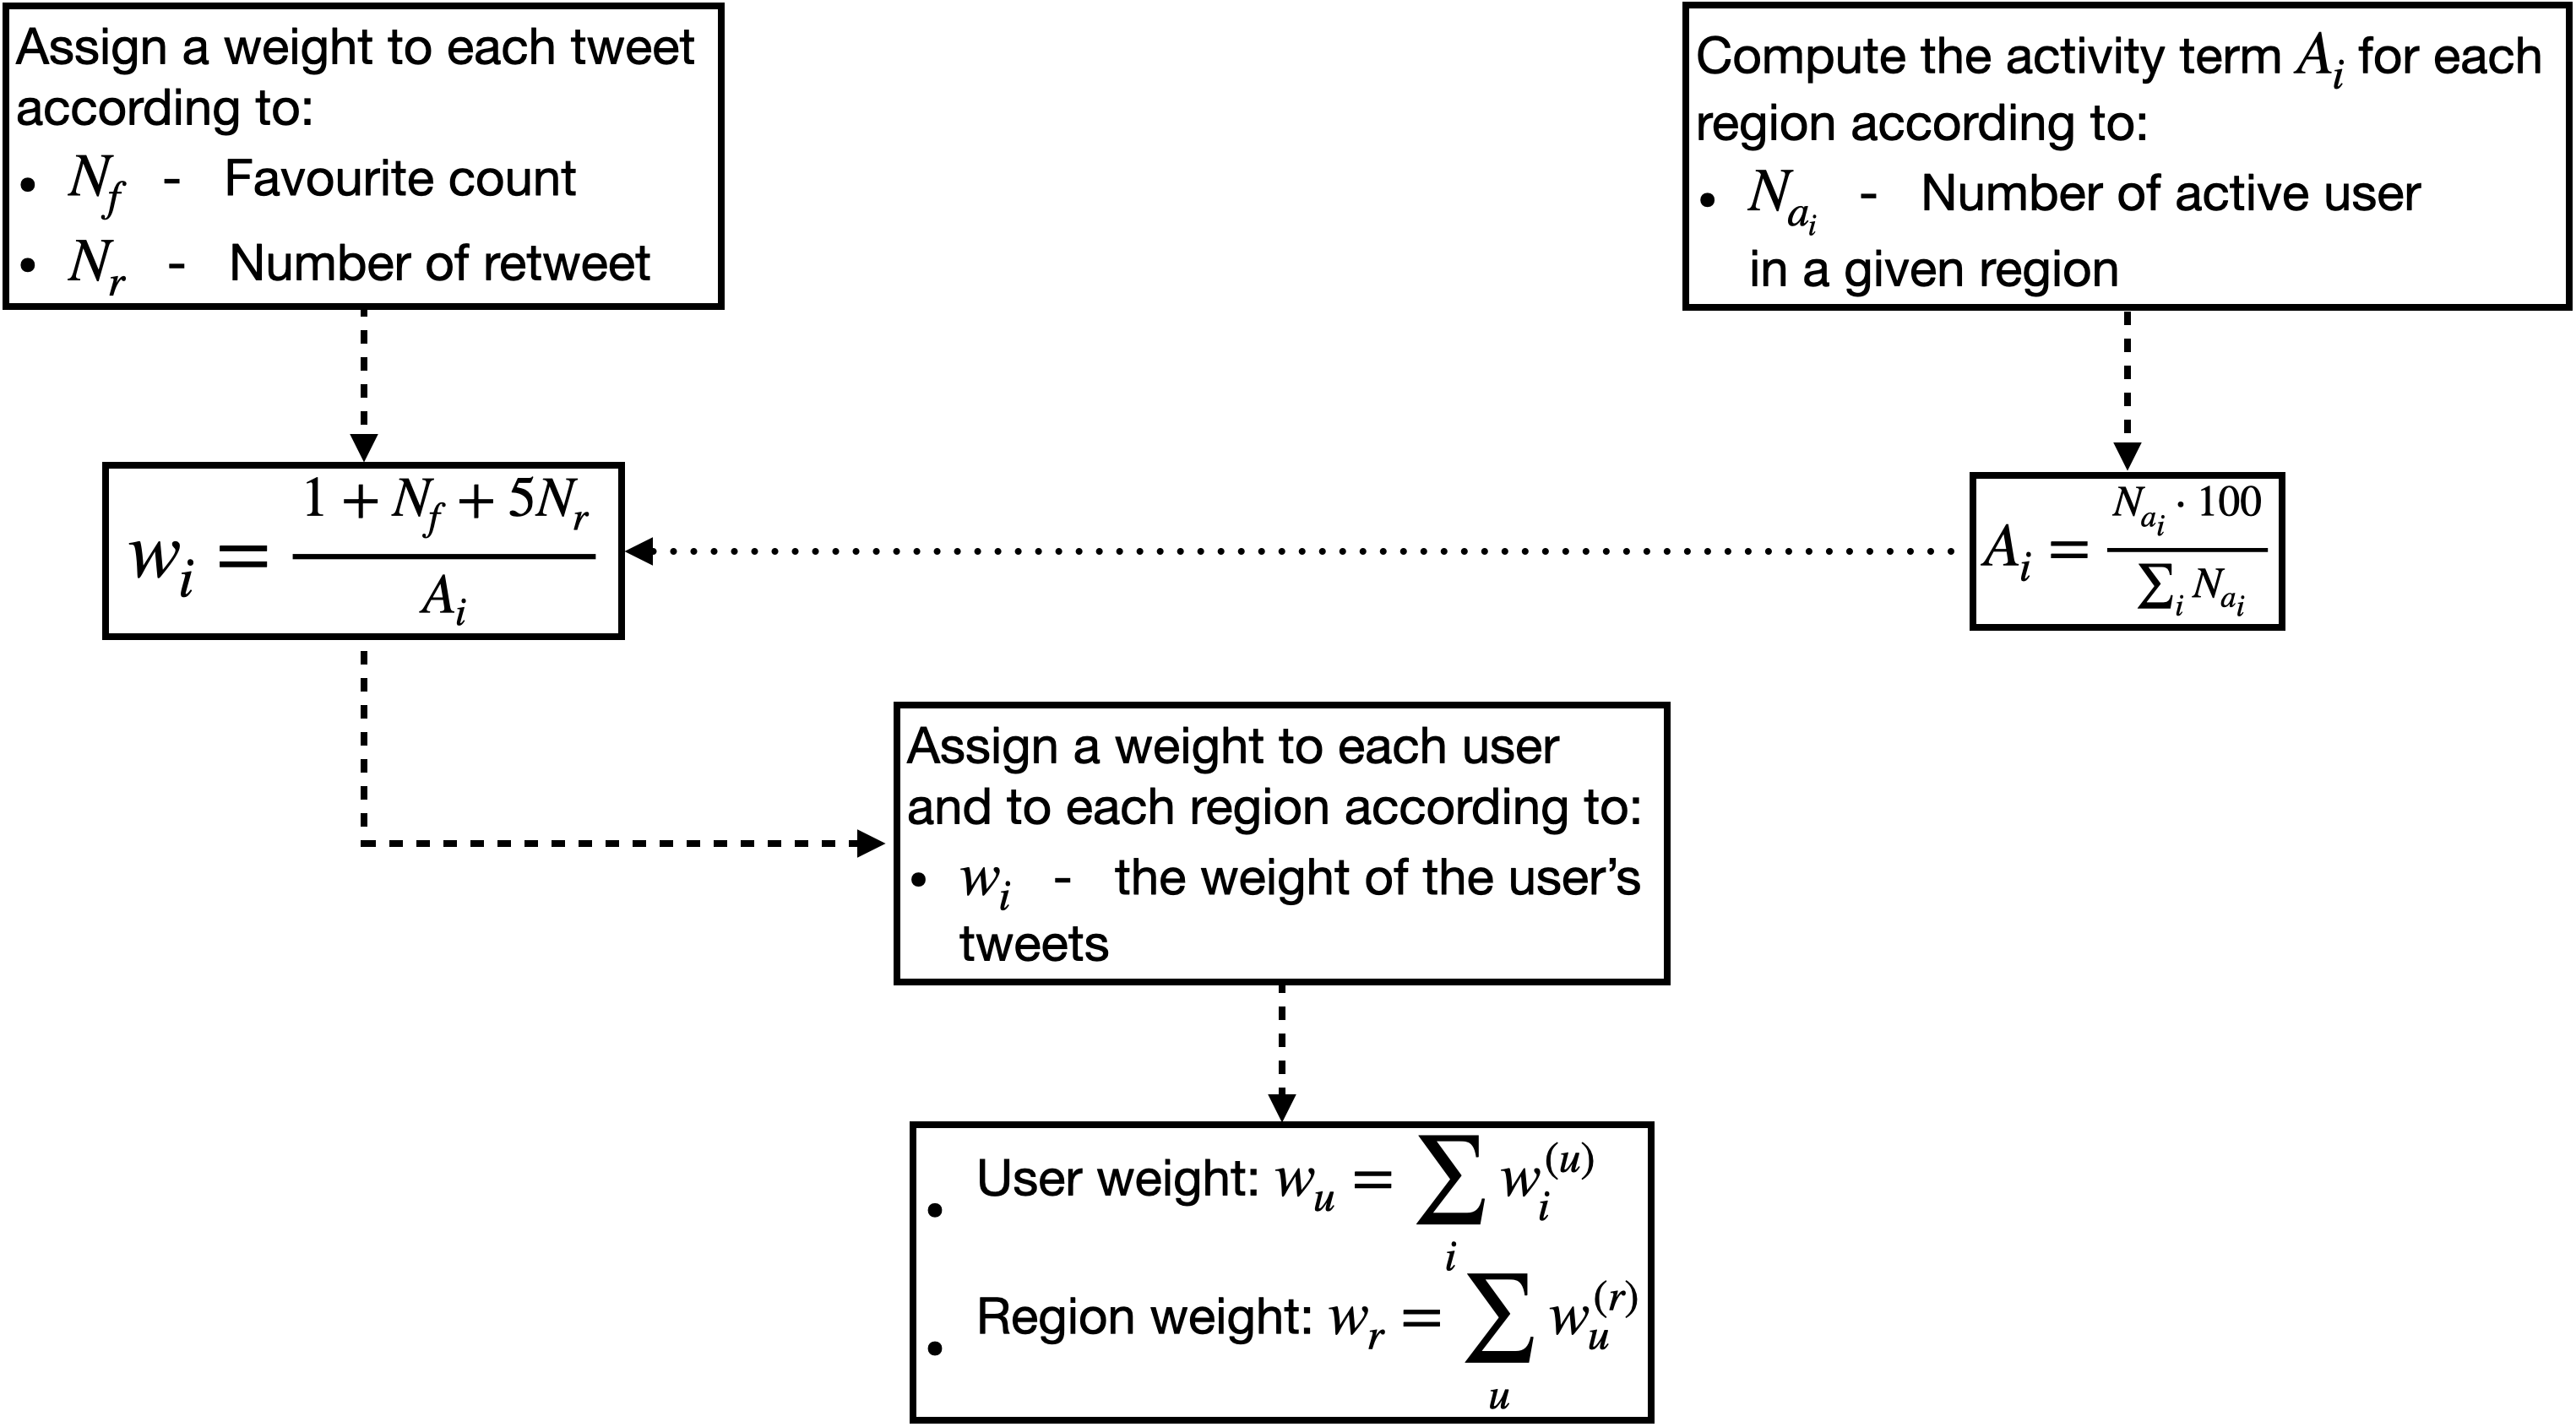
\includegraphics[width=1\textwidth]{images/schema.png}
   \label{fig:count_word}
   \end{minipage}
    \end{figure}
	
	\end{frame}
	
	\section{Critical Issues}
	
	\begin{frame}[c]{Critical Issues}
	\framesubtitle{Aspects to be improved}

	\boxed{\textbf{Amount of data}}

	\medskip
	Our capability of collecting useful data is \alert{limited} by the \alert{free version of the Twitter API}
	
	\medskip
	$\implies$ highly biased results.
	
	\medskip
	\medskip
	\pause
	\boxed{\textbf{Manual work}}
	
	\medskip
	We perform some tasks without automation
	
	\medskip
	
	$\implies$ having \alert{more data means automating all processes}.
	
	\medskip
	\medskip
	\pause
	\boxed{\textbf{Different weights}}
	
	\medskip
	Consider different ways to assign weights to each tweet to produce more complex analysis
	
	\medskip
	
	$\implies$ compare the activity data with the population to produce the normalization term.
	
	\end{frame}
	
	\section{Results}
	\begin{frame}{Results}
	    \framesubtitle{Most frequent words distribution}
	    \begin{figure}[t]
	    \begin{minipage}[l]{1\columnwidth}
	    \centering
	    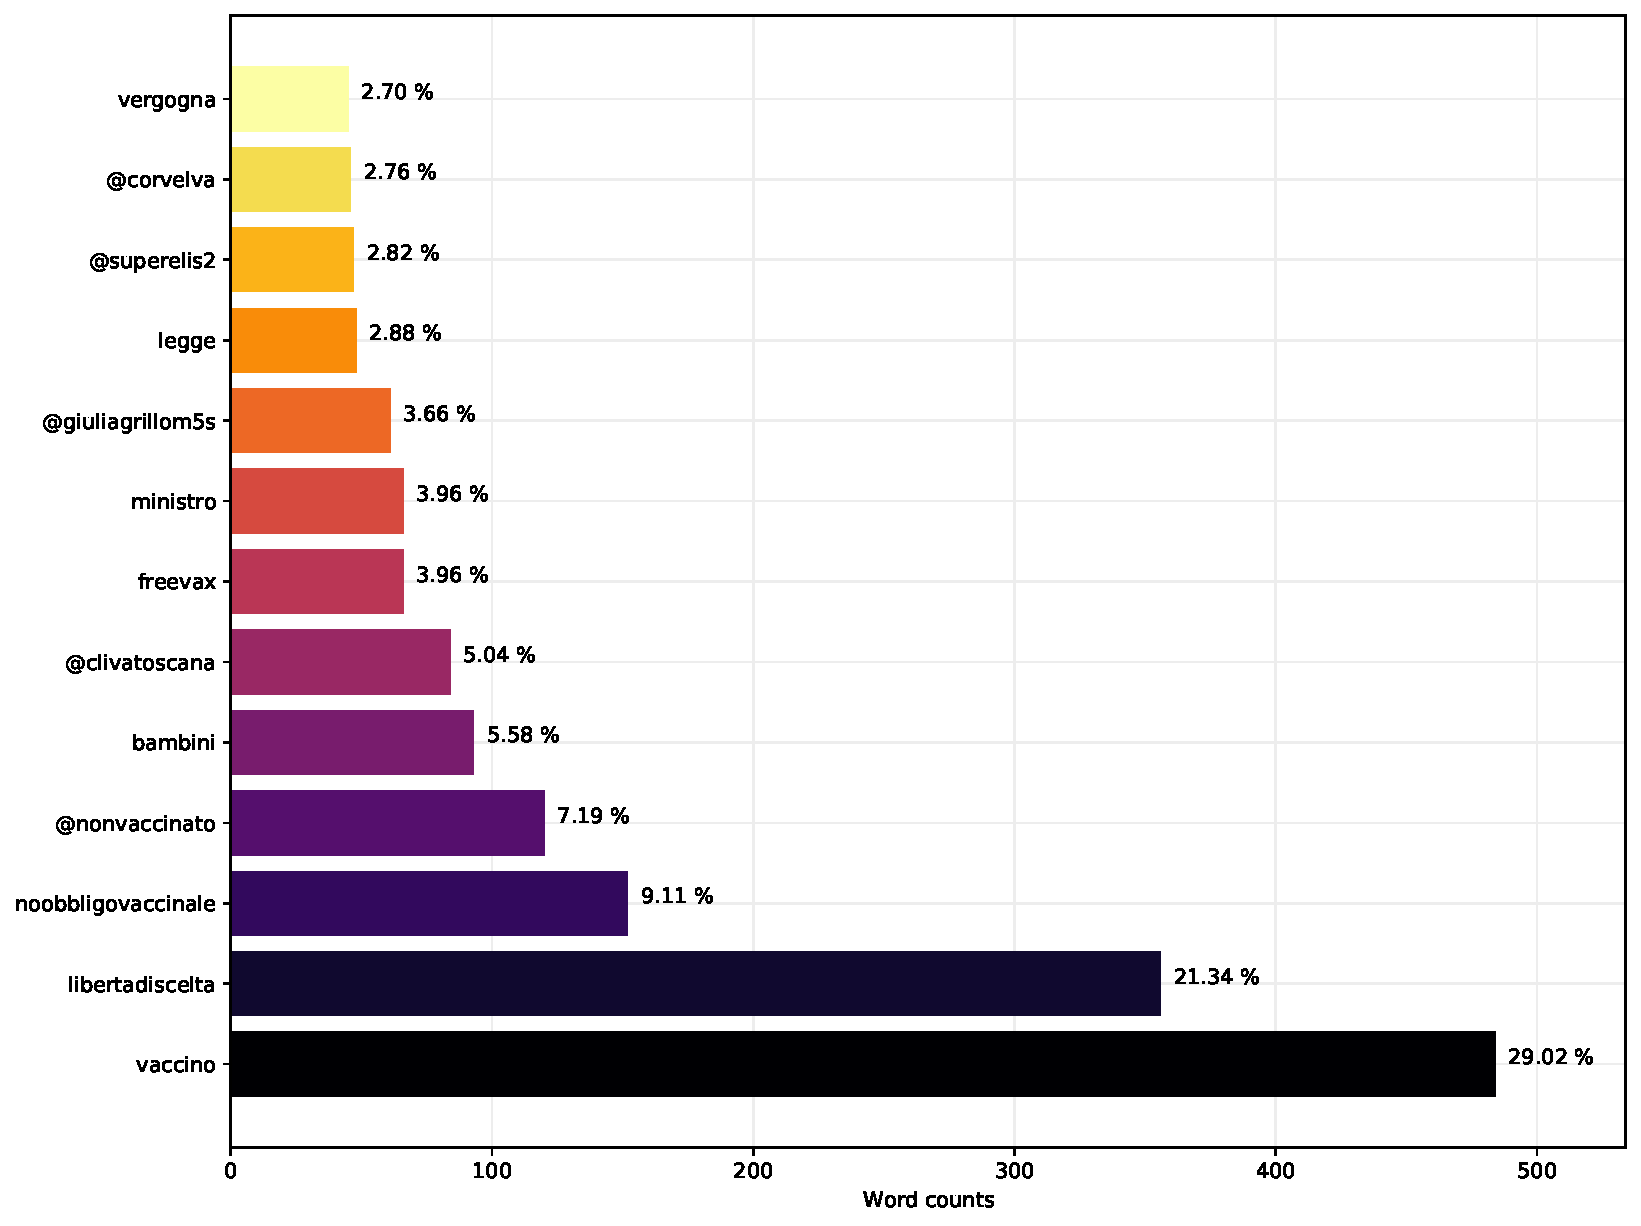
\includegraphics[width=0.7\textwidth]{images/word_2017-2020.pdf}
	    \caption{Histogram of most used words in the novax collected tweets in 2017-2020.}
   \label{fig:count_word}
   \end{minipage}
\end{figure}
	
	\end{frame}
	
	\begin{frame}{Results}
	    \framesubtitle{User overlap}
\begin{figure}[t]
   \begin{minipage}[l]{1.0\columnwidth}
   \centering
   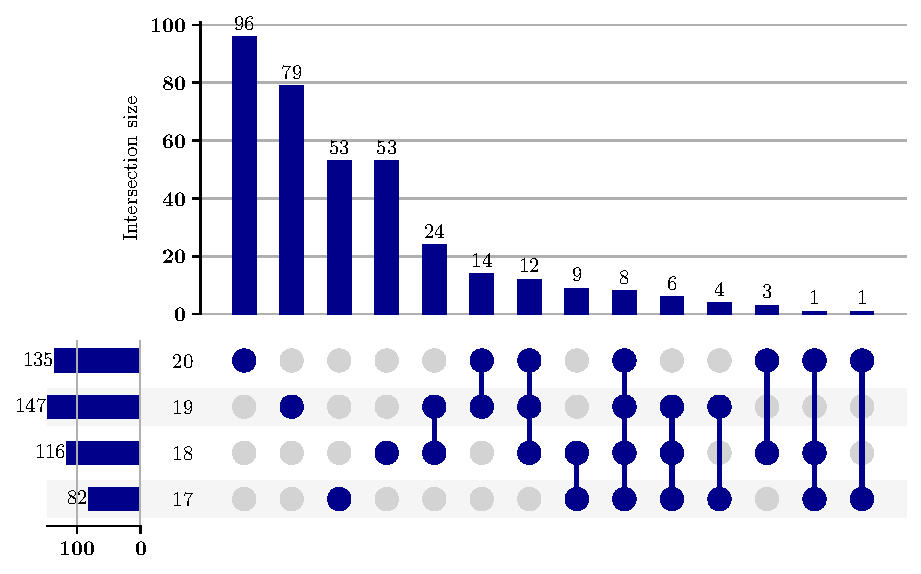
\includegraphics[width=0.7\textwidth]{images/overlap.pdf}
   \caption{Twitter user overlap between 2017, 2018, 2019 and 2020.}
   \label{fig:overlap}
   \end{minipage}
\end{figure}
	
	\end{frame}



\begin{frame}{Results}
\framesubtitle{Numbers: Twitter activity by region and vaccination coverage}

 \begin{table}[b]
 \tiny
    \begin{minipage}[l]{0.4\textwidth}
    %\centering
        \begin{tabular*}{\linewidth}{@{\extracolsep{\fill}} l c c c}
       \textbf{Region}	&	\textbf{$I$}	&	\textbf{$A$} &	\textbf{$\frac{I- A}{I}$}	\\
 \colrule
       & & & \\
Prov. Au. di Bolzano	&	0.9	&	0.2	&	0.7	\\
Molise	&	0.5	&	0.2	&	0.6	\\
Sicilia	&	8.2	&	5.5	&	0.3	\\
Puglia	&	6.6	&	4.5	&	0.3	\\
Prov. Au. di Trento	&	0.9	&	0.6	&	0.3	\\
Calabria	&	3.2	&	2.3	&	0.3	\\
Campania	&	9.6	&	7.3	&	0.2	\\
Basilicata	&	0.9	&	0.7	&	0.2	\\
Friuli Venezia Giulia	&	2.0	&	1.6	&	0.2	\\
Veneto	&	8.2	&	6.6	&	0.2	\\
Abruzzo	&	2.2	&	1.8	&	0.2	\\
Sardegna	&	2.7	&	2.4	&	0.1	\\
Valle d'Aosta	&	0.2	&	0.2	&	0.1	\\
Piemonte	&	7.2	&	7.1	&	0.0	\\
Umbria	&	1.5	&	1.5	&	0.0	\\
Marche	&	2.5	&	2.7	&	-0.1	\\
Emilia Romagna	&	7.5	&	8.5	&	-0.1	\\
Lombardia	&	16.8	&	19.2	&	-0.1	\\
Toscana	&	6.2	&	7.5	&	-0.2	\\
Liguria	&	2.6	&	3.4	&	-0.3	\\
Lazio	&	9.7	&	16.0	&	-0.7	\\

        \end{tabular*}
    \caption{Inhabitants / Twitter activity 
    comparison}
    \label{tab:inhab-activity}
    \end{minipage}
    \hspace{1cm} %bastava eliminare gli spazi s? <3 si ahahha <3 <3 <3
    \begin{minipage}[l]{0.4\textwidth}
    %\centering
        \begin{tabular*}{\linewidth}{@{\extracolsep{\fill}} l c c c}
       \textbf{Region}	&	\textbf{2017}	&	\textbf{2018}	&	\textbf{2019}	\\
      % \hline
      & & & \\
Abruzzo	&	89.20	&	94.49	&	95.05	\\
Basilicata	&	92.90	&	92.98	&	92.57	\\
Calabria	&	92.79	&	92.72	&	93.08	\\
Campania	&	92.03	&	93.39	&	94.67	\\
Emilia Romagna	&	93.48	&	93.67	&	95.21	\\
Friuli Venezia Giulia	&	86.55	&	91.24	&	92.49	\\
Lazio	&	95.34	&	94.87	&	95.72	\\
Liguria	&	90.92	&	94.04	&	93.15	\\
Lombardia	&	93.92	&	94.16	&	95.56	\\
Marche	&	88.21	&	92.07	&	93.75	\\
Molise	&	90.48	&	91.95	&	93.39	\\
Piemonte	&	94.72	&	94.67	&	95.56	\\
Prov. Au. di Bolzano	&	71.86	&	70.84	&	75.53	\\
Prov. Au. di Trento	&	91.68	&	94.30	&	95.48	\\
Puglia	&	91.09	&	94.18	&	94.38	\\
Sardegna	&	93.00	&	92.33	&	93.61	\\
Sicilia	&	85.63	&	90.94	&	92.20	\\
Toscana	&	93.51	&	95.04	&	96.11	\\
Umbria	&	94.53	&	94.59	&	95.23	\\
Valle d'Aosta	&	90.33	&	91.43	&	91.54	\\
Veneto	&	92.34	&	93.49	&	95.12	\\
Italian average & 91.84 & 93.22 & 94.49 \\
        \end{tabular*}
    \label{tab:inhab-activity}
    \caption{Measles vaccination coverage \\ 
    2 years after birth}
    \label{tab:inhab-activity}
    \end{minipage}
    \end{table}
    
    
\end{frame}


\begin{frame}{Results}
\framesubtitle{Maps: vaccination coverage and Twitter novax activity by region}
	% To insert four subfigure
	\begin{figure}
	\begin{minipage}[c]{0.48\linewidth}
	\centering
	\subfloat[][2017]{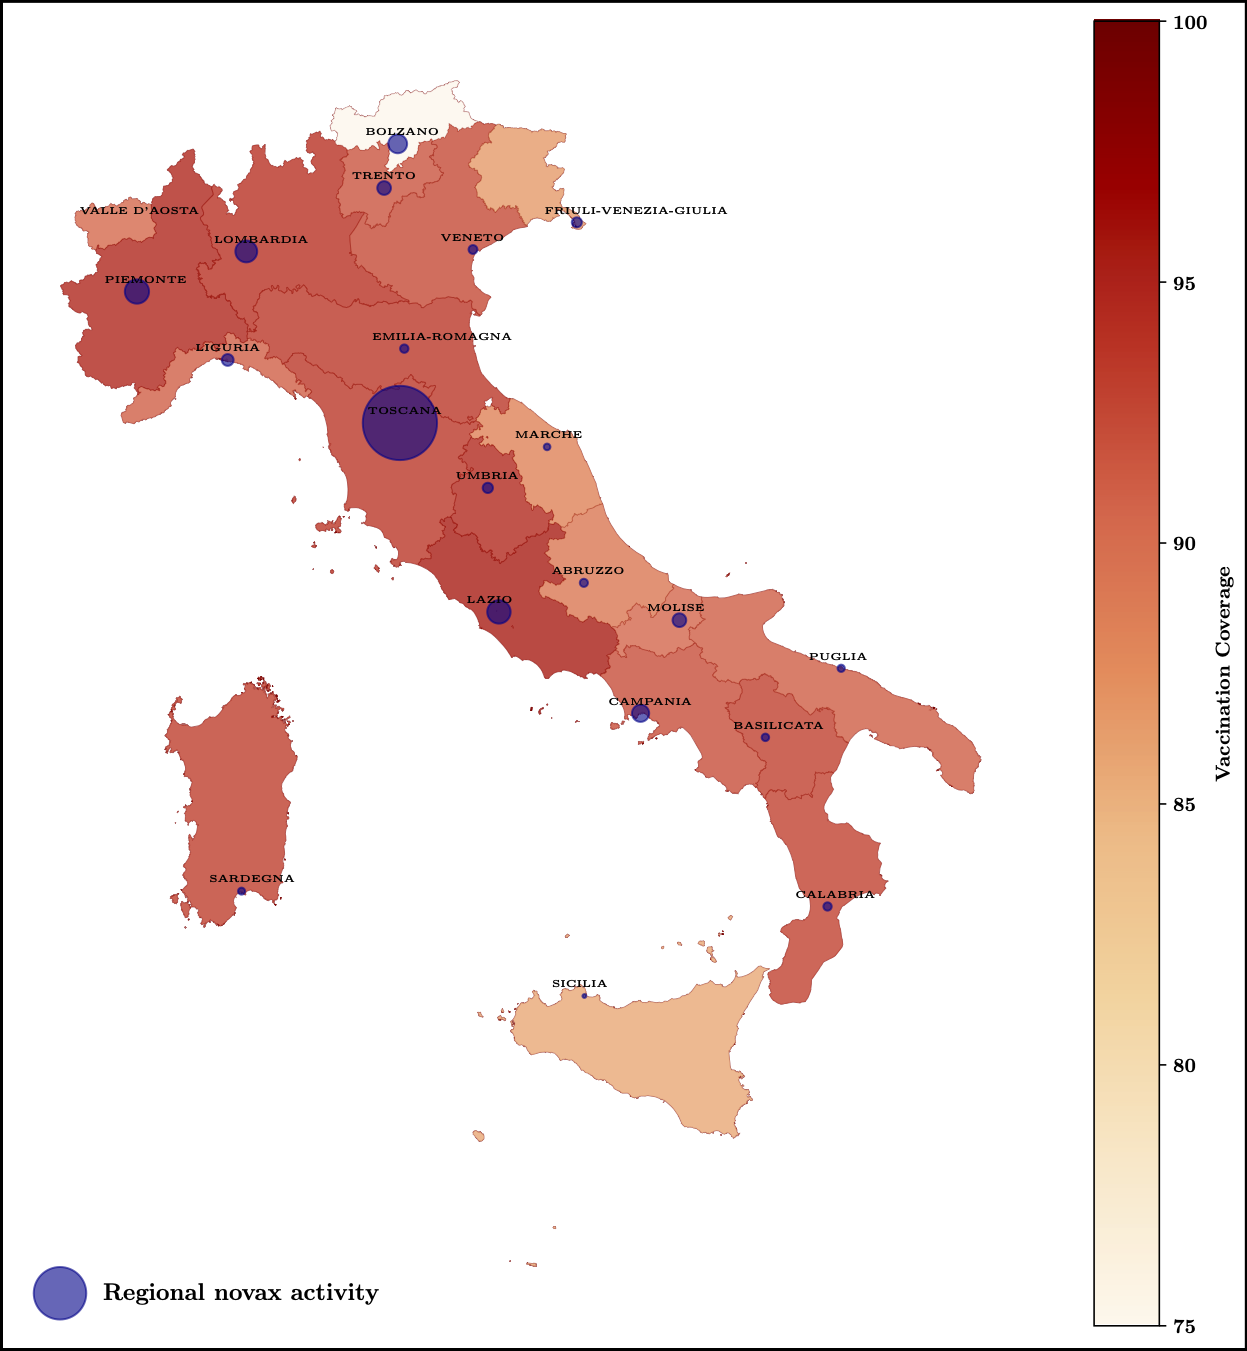
\includegraphics[width=1\textwidth]{images/map_2017.png} \label{fig:map_result_a} }
	\end{minipage}
	\begin{minipage}[]{0.48\linewidth}
	\centering
	\subfloat[][2018]{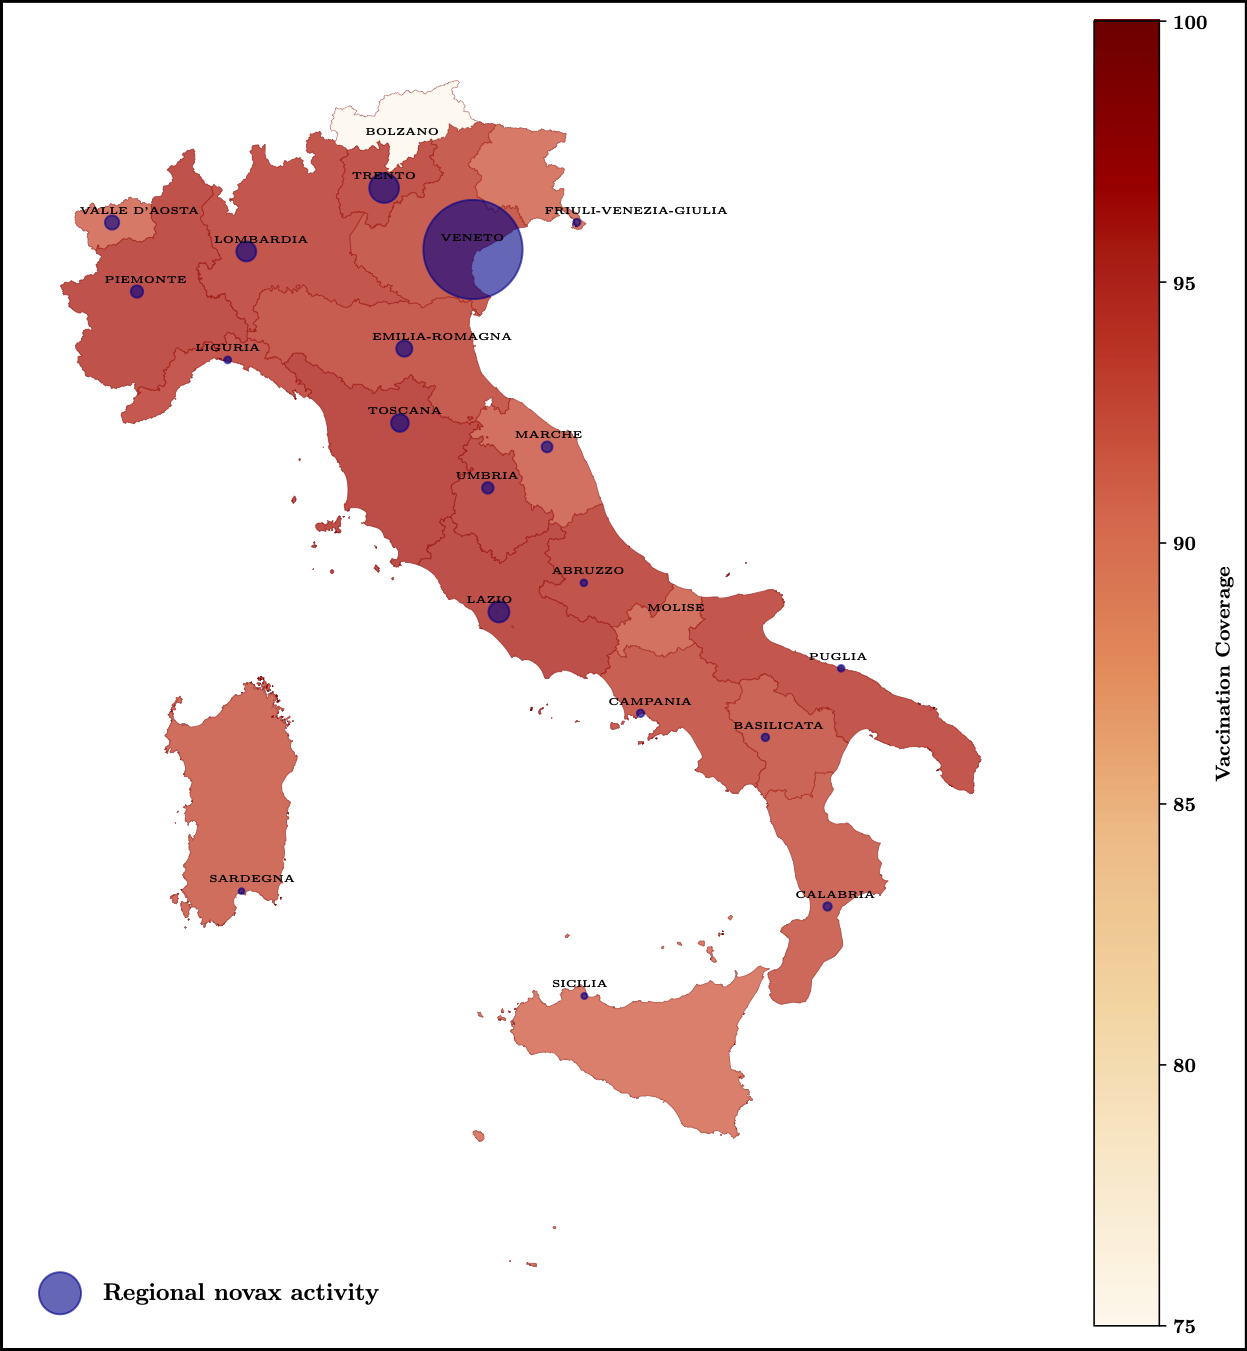
\includegraphics[width=1\textwidth]{images/map_2018.png} \label{fig:map_result_b} }
	\end{minipage} 
	\caption{Overlap between measles vaccination coverage and Twitter novax activity}
	\end{figure}
	\end{frame}
	
	\begin{frame}{Results}
\framesubtitle{Maps: vaccination coverage and Twitter novax activity by region}

\begin{figure}
	\begin{minipage}[c]{0.48\linewidth}
	\centering
	\subfloat[][2019]{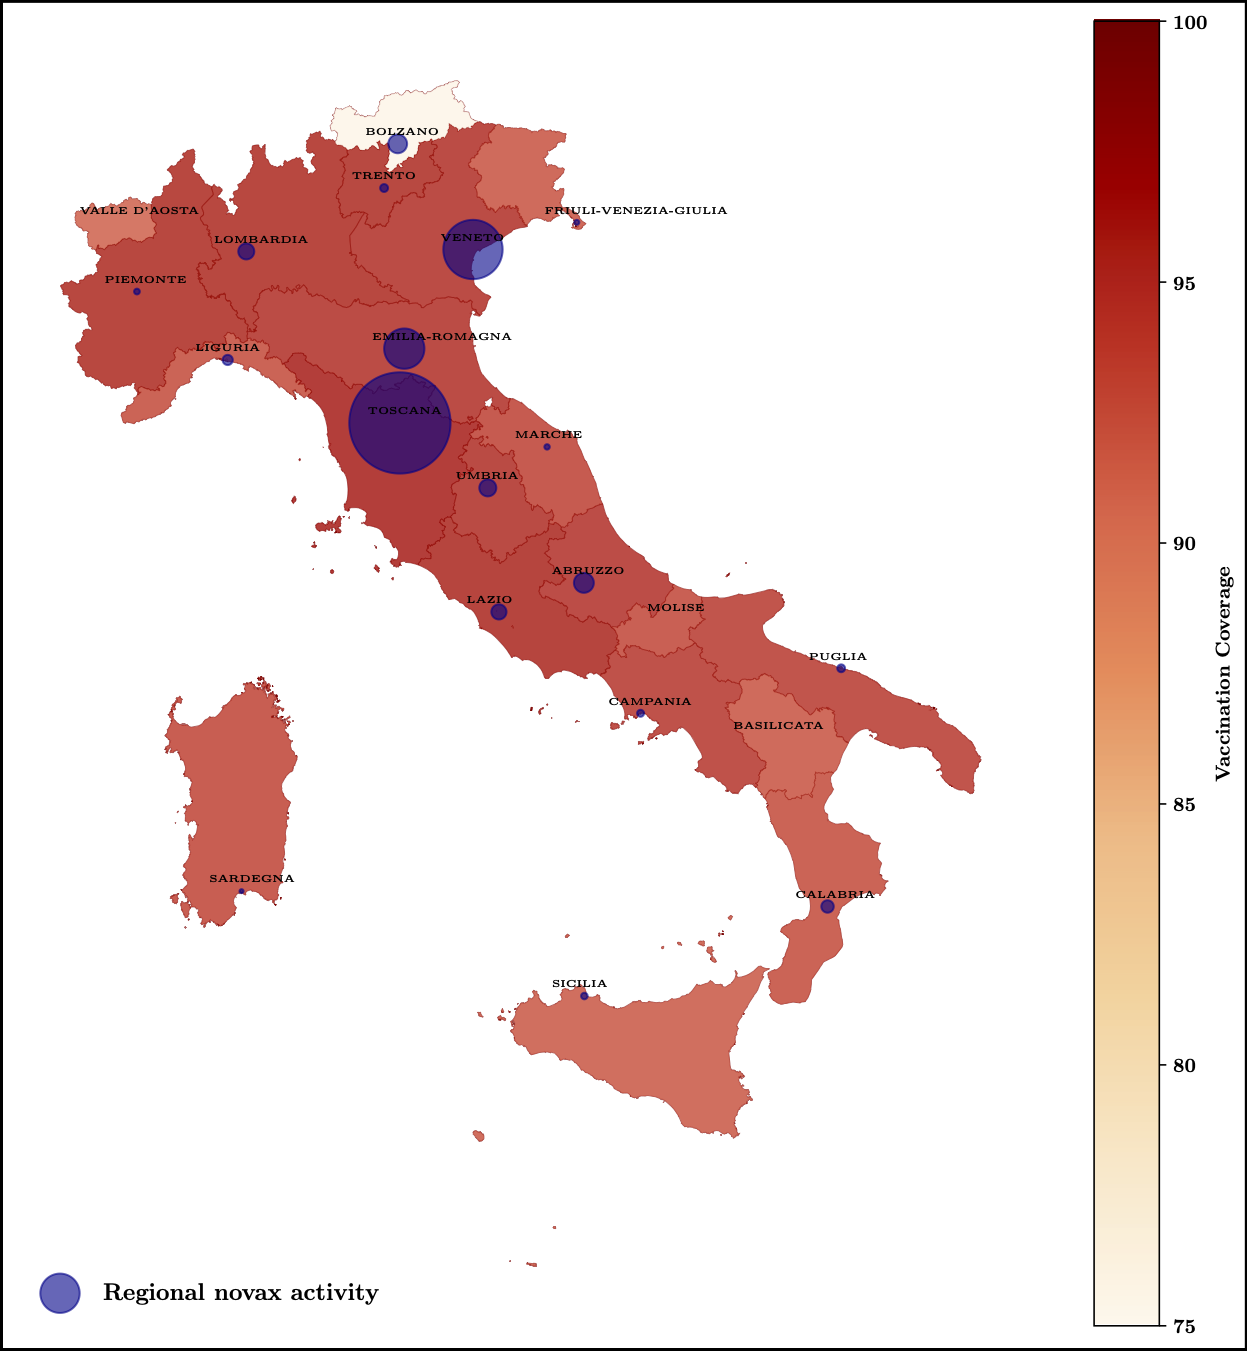
\includegraphics[width=1\textwidth]{images/map_2019.png} \label{fig:map_result_b} }
	\end{minipage} 
	\begin{minipage}[c]{0.48\linewidth}
	\centering
	\subfloat[][2020]{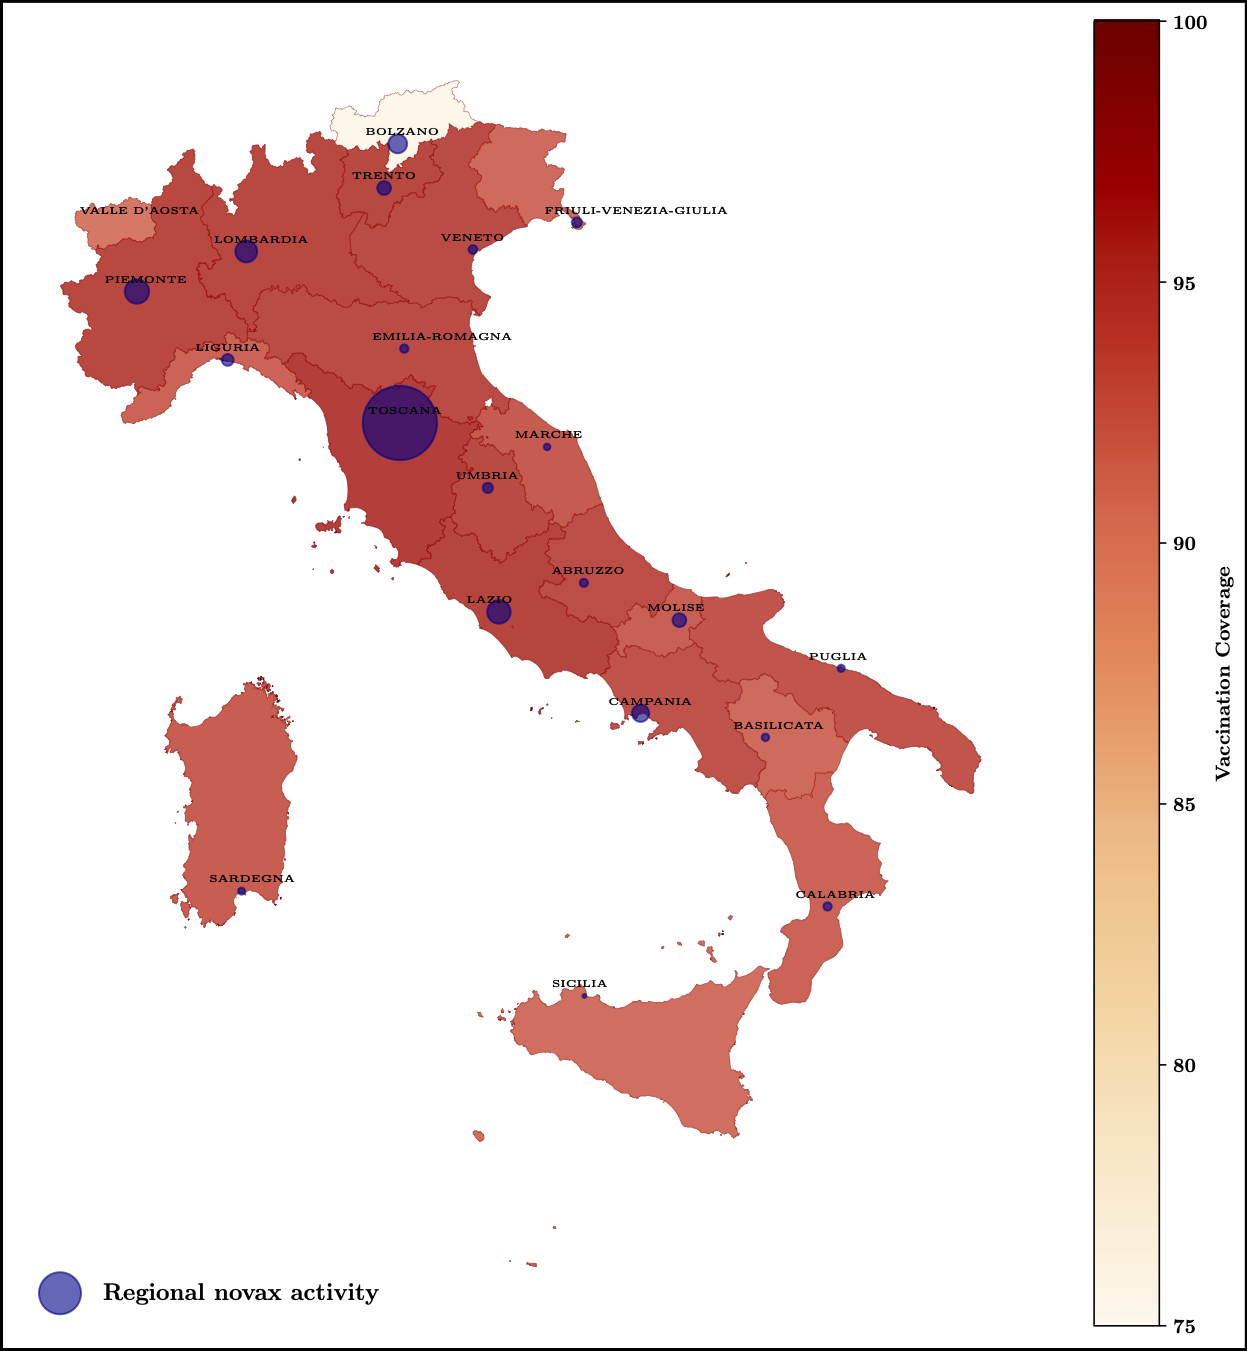
\includegraphics[width=1\textwidth]{images/map_2020.png} \label{fig:map_result_c} }
	\end{minipage}
	\caption{Overlap between measles vaccination coverage and Twitter novax activity}
	\end{figure}
	\end{frame}
	
%	\begin{figure}
 %   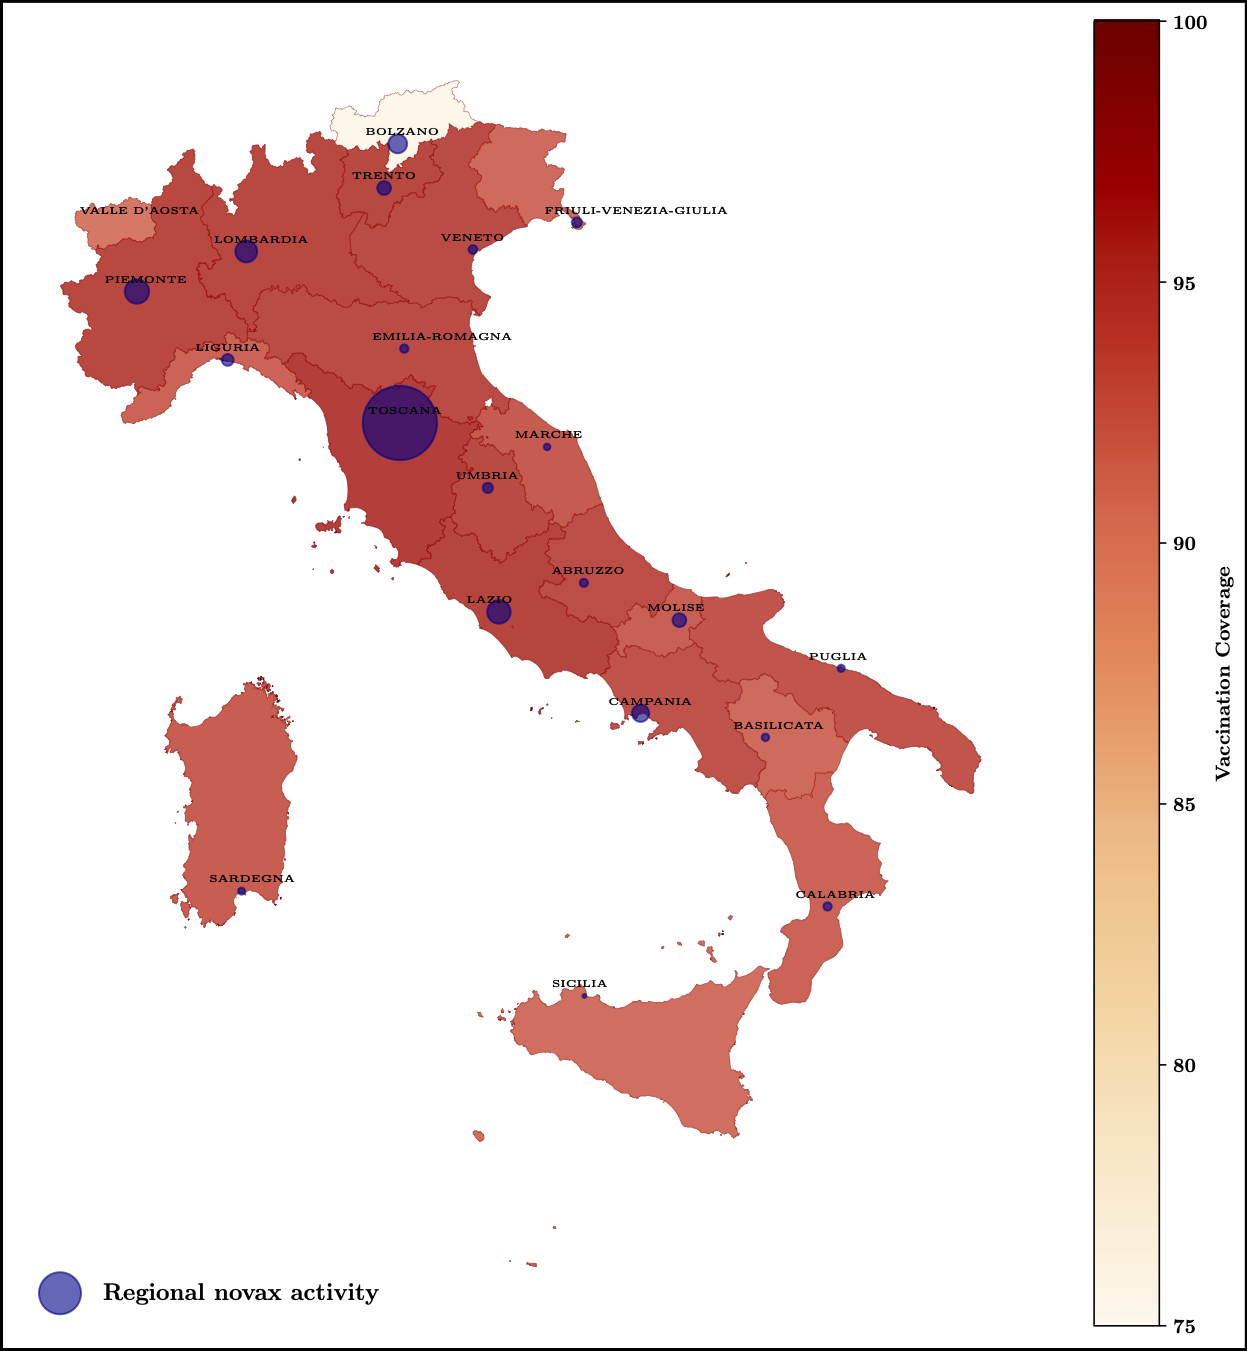
\includegraphics[width=0.5\textwidth]{images/map_2020.png} 
    %\vspace{1cm}
%	\caption{Overlap between measles vaccination coverage and Twitter novax activity in 2020}
%	\end{figure}


\section{Conclusion}
\begin{frame}{Conclusion}
	   \framesubtitle{~} % DA LASCIARE! NON COMMENTARE

	 \begin{block}{}\centering We present a method to analyze the geographical distribution\\ of novax opinions by means of tweets with anti-vaccine content.\end{block}

	\medskip
	
	\pause
	We study the novax distribution in the time interval 2017-2020 in Italy.
	
	\medskip
	
	The analysis results are:
	
	\medskip
	
	\begin{itemize}
	    \item some \alert{super spreaders} create original tweets, which are retweeted by the majority;
	    
	    \item in \alert{2020} there are more \alert{new users} with respect to the past years, probably as a consequence of Covid-19; 
	    
	    \item \alert{map results}: some local hubs due to super spreaders, constant distribution of novax opinion over the years, no correspondence between low coverage and novax hubs.
	   
	\end{itemize}
	
	\medskip
	
	To confirm all these hypothesis with a meaningful confidence level, \alert{many more data} would have been required.
	\end{frame}
	
	
\begin{frame}{Conclusion}
	    \framesubtitle{Further analysis and possible applications}
	
	\boxed{\textbf{Further analysis}} \\
	\medskip
	\begin{itemize}
	    \item Collect a greater number of data to make an \alert{analysis at province level}
	    
	    \item Create a \alert{network} by making links between original tweets and their retweets
	    
	    \item Make an analogous analysis on \alert{other social networks} with a different audience to increase statistics and data reliability
	    
	\end{itemize}
	\pause
	 \vspace{1cm}
	 
	\boxed{\textbf{Applications}} 
	\medskip
	
	Identify hubs of anti-vaccination ideas 
	
	\medskip

	$\implies$ choose where to invest resources for awareness campaigns on vaccination.


	\end{frame}
\usebackgroundtemplate{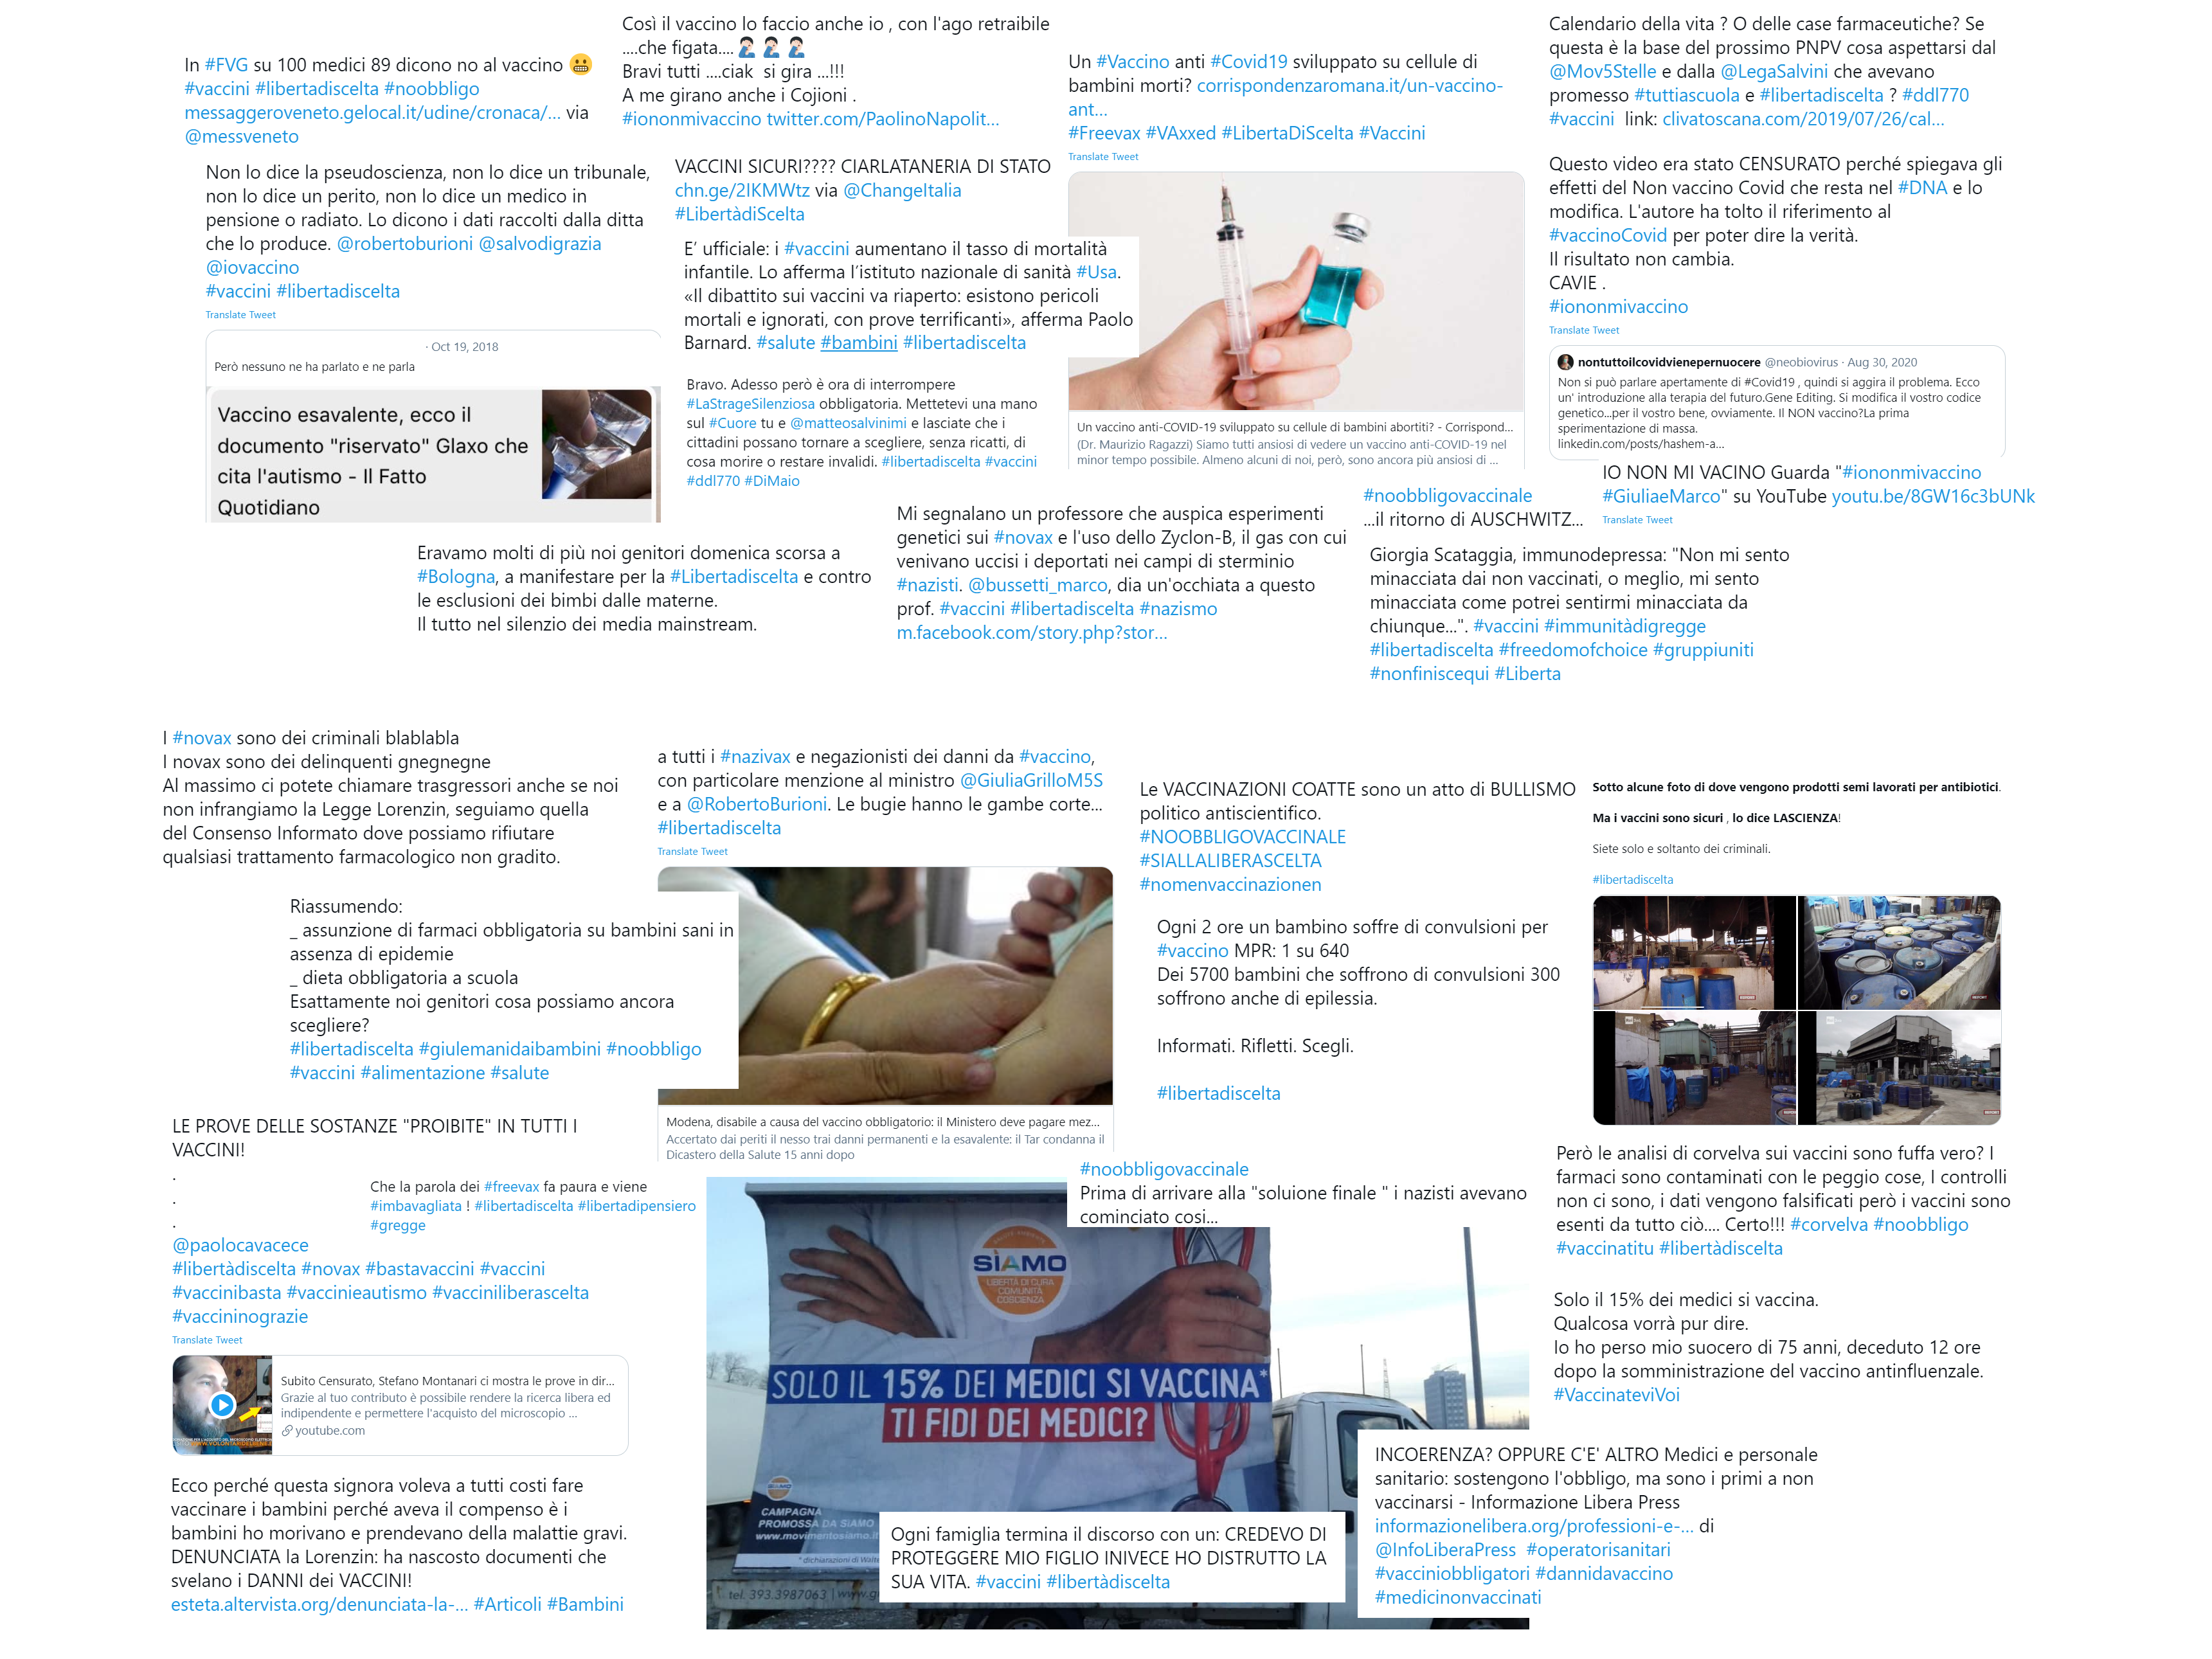
\includegraphics[width=\paperwidth]{Alldef.png}}	
\begin{frame}
 %\framesubtitle{~}
 \vspace{0.32cm}
	\centering
\huge{So long and thanks for all the fish}    
	

\end{frame}
	


\end{document}